\documentclass[11pt,a4paper]{article}

\usepackage[T1]{fontenc}
\usepackage[utf8]{inputenc}
\usepackage{lmodern}
\usepackage{microtype}
\usepackage{amsmath,amssymb,mathtools}
\usepackage{graphicx}
\usepackage{booktabs}
\usepackage{enumitem}
\usepackage{xcolor}
\usepackage{geometry}
\usepackage{hyperref}

\geometry{margin=2.2cm}
\graphicspath{{../figures/}}
\hypersetup{colorlinks=true,linkcolor=blue!50!black,urlcolor=blue!50!black}
\setlength{\parindent}{0pt}
\setlength{\parskip}{0.45em}

\definecolor{accent}{RGB}{22,63,117}

\newcommand{\R}{\mathbb{R}}
\newcommand{\E}{\mathbb{E}}
\newcommand{\Var}{\mathrm{Var}}
\newcommand{\Cov}{\mathrm{Cov}}
\newcommand{\Dt}{\Delta_t}
\newcommand{\pt}{p_t}
\newcommand{\Ht}{\mathcal{H}_t}
\newcommand{\diag}{\mathrm{diag}}
\newcommand{\PhiN}{\Phi}

\title{\vspace{-1.1cm}\textbf{\color{accent}Diffused Laplace AR(1):}\\[2mm]
\Large exact $K=1$ benchmark, nonlinear score, and state-dependent effective precision}
\author{}
\date{March 2026}

\begin{document}
\maketitle
\vspace{-1.6em}

\begin{center}
\setlength{\fboxsep}{8pt}
\fcolorbox{accent!35}{accent!4}{%
\begin{minipage}{0.95\textwidth}
\textbf{Hypothesis -> derivation -> signal -> conclusion.}
\begin{enumerate}[leftmargin=1.35em,itemsep=0.2em,topsep=0.2em]
\item \textbf{Hypothesis.} Relative to the Gaussian benchmark, the first robust non-Gaussian signal should be that $-\nabla^2 \log \pt(x)$ is no longer constant.
\item \textbf{Derivation.} For $K=1$, the Laplace model admits an exact one-dimensional reduction after OU noising. From it one gets closed formulas for the density, the score, and the curvature matrix $\Ht(x):=-\nabla_x^2 \log \pt(x)$.
\item \textbf{Signal.} The score is nonlinear and $\Ht(x)$ varies with $x$.
\item \textbf{Conclusion.} Finite-time smoothing does \emph{not} Gaussianize the Laplace model. The old draft's stronger $K=2$ ``closed-form'' claim is not retained.
\end{enumerate}
\end{minipage}}
\end{center}

\section{Model and the benchmark question}

We study the two-frame Laplace AR(1) model
\begin{equation}
A_0 \sim \mathcal N(\mu_0,\sigma_0^2),
\qquad
A_1 = \alpha A_0 + \varepsilon,
\qquad
\varepsilon \sim \mathrm{Laplace}(0,b),
\qquad |\alpha|<1,
\label{eq:model-clean}
\end{equation}
followed by independent OU noising
\begin{equation}
X_k = e^{-t} A_k + \sqrt{\Dt} \, Z_k,
\qquad
\Dt = 1-e^{-2t},
\qquad
Z_0,Z_1 \stackrel{\mathrm{iid}}{\sim} \mathcal N(0,1).
\label{eq:ou-noising}
\end{equation}

The matched Gaussian reference replaces $\varepsilon$ by $\varepsilon_G \sim \mathcal N(0,2b^2)$, so the clean first two moments match exactly. In that Gaussian model,
\begin{equation}
\nabla \log p_t^{\mathrm G}(x) = -Q_t(x-\mu_t),
\qquad
-\nabla^2 \log p_t^{\mathrm G}(x) \equiv Q_t,
\label{eq:gaussian-baseline}
\end{equation}
where $Q_t$ is the noisy precision matrix. The whole Gaussian geometry is constant in $x$.

The question is therefore simple:
\begin{quote}
\textbf{After finite OU smoothing, does the Laplace model still retain enough structure for $-\nabla^2 \log \pt(x)$ to depend on $x$?}
\end{quote}

\section{Minimal Gaussian baseline}

For the matched Gaussian model the clean mean and covariance are
\begin{equation}
m_A =
\begin{pmatrix}
\mu_0 \\
\alpha \mu_0
\end{pmatrix},
\qquad
\Sigma_A =
\begin{pmatrix}
\sigma_0^2 & \alpha \sigma_0^2 \\
\alpha \sigma_0^2 & \alpha^2 \sigma_0^2 + 2b^2
\end{pmatrix}.
\label{eq:gaussian-clean}
\end{equation}
After OU noising,
\begin{equation}
\mu_t = e^{-t} m_A,
\qquad
\Sigma_t = e^{-2t} \Sigma_A + \Dt I_2,
\qquad
Q_t = \Sigma_t^{-1}.
\label{eq:gaussian-noisy}
\end{equation}
Hence the benchmark curvature is exactly constant:
\[
\Ht^{\mathrm G}(x) \equiv Q_t.
\]
This is the object that the Laplace model has to beat.

\section[Exact K=1 Laplace reduction]{Exact $K=1$ Laplace reduction}

\subsection*{Step 1: the noised innovation kernel}

Let $\beta_t = e^{-t} b$. The diffused innovation $e^{-t}\varepsilon + \sqrt{\Dt}Z$ has density
\begin{equation}
h(y;\beta_t,\Dt)
=
\frac{e^{\Dt/(2\beta_t^2)}}{2\beta_t}
\left[
 e^{-y/\beta_t}\PhiN\!\left(\frac{y}{\sqrt{\Dt}}-\frac{\sqrt{\Dt}}{\beta_t}\right)
 +
 e^{y/\beta_t}\PhiN\!\left(-\frac{y}{\sqrt{\Dt}}-\frac{\sqrt{\Dt}}{\beta_t}\right)
\right].
\label{eq:normal-laplace}
\end{equation}
This is the exact Laplace-Gaussian convolution. It is smooth for every $t>0$, but it is not Gaussian at finite time.

\begin{figure}[t]
\centering
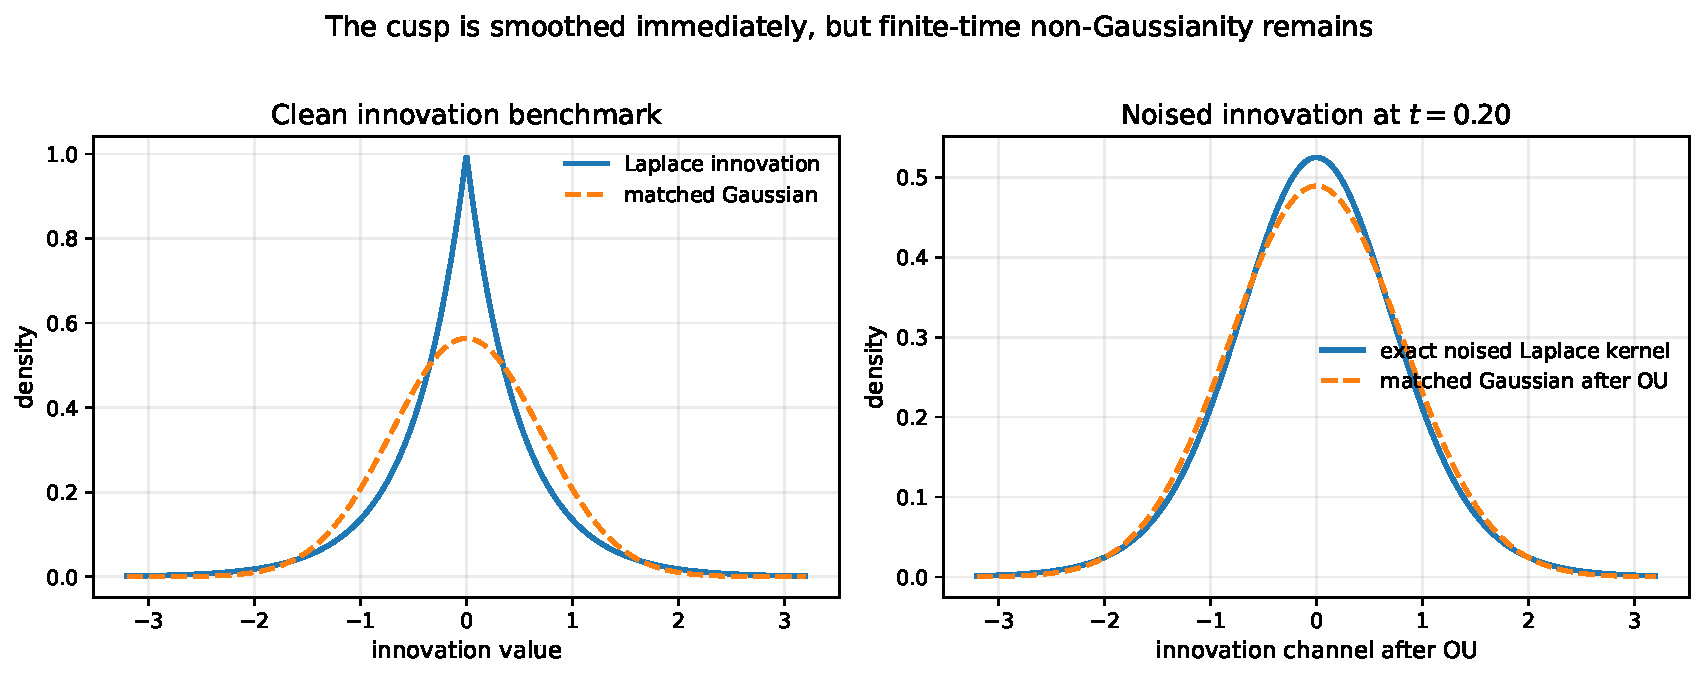
\includegraphics[width=0.94\textwidth]{fig01_innovations_and_kernel.pdf}
\caption{\textbf{Innovation-level benchmark.} Left: the clean Laplace innovation and the matched Gaussian innovation with the same variance $2b^2$. Right: the exact noised innovation density $h(y;\beta_t,\Dt)$ at $t=0.20$. OU noise smooths the cusp immediately, but the finite-time law is still not Gaussian. Parameters: $\alpha=0.8$, $b=0.5$, $\mu_0=0$, and $\sigma_0^2=2b^2/(1-\alpha^2)$.}
\label{fig:kernel}
\end{figure}

\subsection*{Step 2: condition on the first coordinate}

The first noisy coordinate is Gaussian:
\begin{equation}
X_0 \sim \mathcal N(e^{-t}\mu_0, v_x),
\qquad
v_x = e^{-2t}\sigma_0^2 + \Dt.
\label{eq:x0-marginal}
\end{equation}
Moreover,
\begin{equation}
A_0 \mid X_0=x_0 \sim \mathcal N(m_t(x_0),v_t),
\qquad
v_t^{-1} = \sigma_0^{-2} + e^{-2t}\Dt^{-1},
\qquad
m_t(x_0) = v_t\left(\frac{\mu_0}{\sigma_0^2} + \frac{e^{-t}x_0}{\Dt}\right).
\label{eq:posterior-a0}
\end{equation}
If $c_t=e^{-t}\alpha$, then the exact noisy density is
\begin{equation}
\pt(x_0,x_1)
=
\phi_{v_x}(x_0-e^{-t}\mu_0)
\; \E\!\left[h(x_1-c_t A_0;\beta_t,\Dt)\,\middle|\, X_0=x_0\right],
\label{eq:exact-density}
\end{equation}
where $\phi_v(u)=\frac{1}{\sqrt{2\pi v}}e^{-u^2/(2v)}$.

So the whole $K=1$ problem is reduced to a \emph{one-dimensional Gaussian expectation}. No Monte Carlo approximation is needed.

\section{Exact score and exact effective precision}

For $r=0,1,2$, define
\begin{equation}
I_r(x_0,x_1;t)
:=
\E\!\left[h^{(r)}(x_1-c_tA_0;\beta_t,\Dt)\,\middle|\, X_0=x_0\right].
\label{eq:Ir-def}
\end{equation}
Then $\pt(x_0,x_1)=\phi_{v_x}(x_0-e^{-t}\mu_0) I_0(x_0,x_1;t)$, and the exact score is
\begin{align}
\partial_{x_1} \log \pt(x_0,x_1)
&= \frac{I_1}{I_0},
\label{eq:score-x1}\\[0.25em]
\partial_{x_0} \log \pt(x_0,x_1)
&= -\frac{x_0-e^{-t}\mu_0}{v_x}
-c_t m_t'(x_0) \frac{I_1}{I_0},
\qquad
m_t'(x_0)=\frac{v_t e^{-t}}{\Dt}.
\label{eq:score-x0}
\end{align}

Now define the effective precision
\begin{equation}
\Ht(x) := -\nabla_x^2 \log \pt(x).
\label{eq:effective-precision-def}
\end{equation}
A direct differentiation gives
\begin{align}
(\Ht(x))_{11}
&= \frac{I_1^2 - I_0 I_2}{I_0^2},
\label{eq:H11}\\[0.25em]
(\Ht(x))_{01}
&= -c_t m_t'(x_0) (\Ht(x))_{11},
\label{eq:H01}\\[0.25em]
(\Ht(x))_{00}
&= \frac{1}{v_x} + c_t^2 \bigl(m_t'(x_0)\bigr)^2 (\Ht(x))_{11}.
\label{eq:H00}
\end{align}
In the Gaussian case these are constants. In the Laplace case they are functions of $x$.

\paragraph{Why this is a genuinely non-Gaussian signal.}
If $\Ht(x)$ were constant on all of $\R^2$, then $\nabla \log \pt(x)$ would be affine, hence $\log \pt(x)$ would be a quadratic polynomial and $\pt$ would be Gaussian. But the exact characteristic function is
\begin{equation}
\Phi_t(\xi_0,\xi_1)
=
\exp\!\Bigl(
 i e^{-t}\mu_0(\xi_0+\alpha\xi_1)
 -\tfrac12 \Dt (\xi_0^2+\xi_1^2)
 -\tfrac12 e^{-2t}\sigma_0^2 (\xi_0+\alpha\xi_1)^2
\Bigr)
\frac{1}{1+b^2 e^{-2t} \xi_1^2},
\label{eq:cf-laplace}
\end{equation}
and the rational factor $(1+b^2 e^{-2t}\xi_1^2)^{-1}$ prevents Gaussianity at every finite $t$. Therefore $\Ht(x)$ cannot be constant.

\begin{figure}[t]
\centering
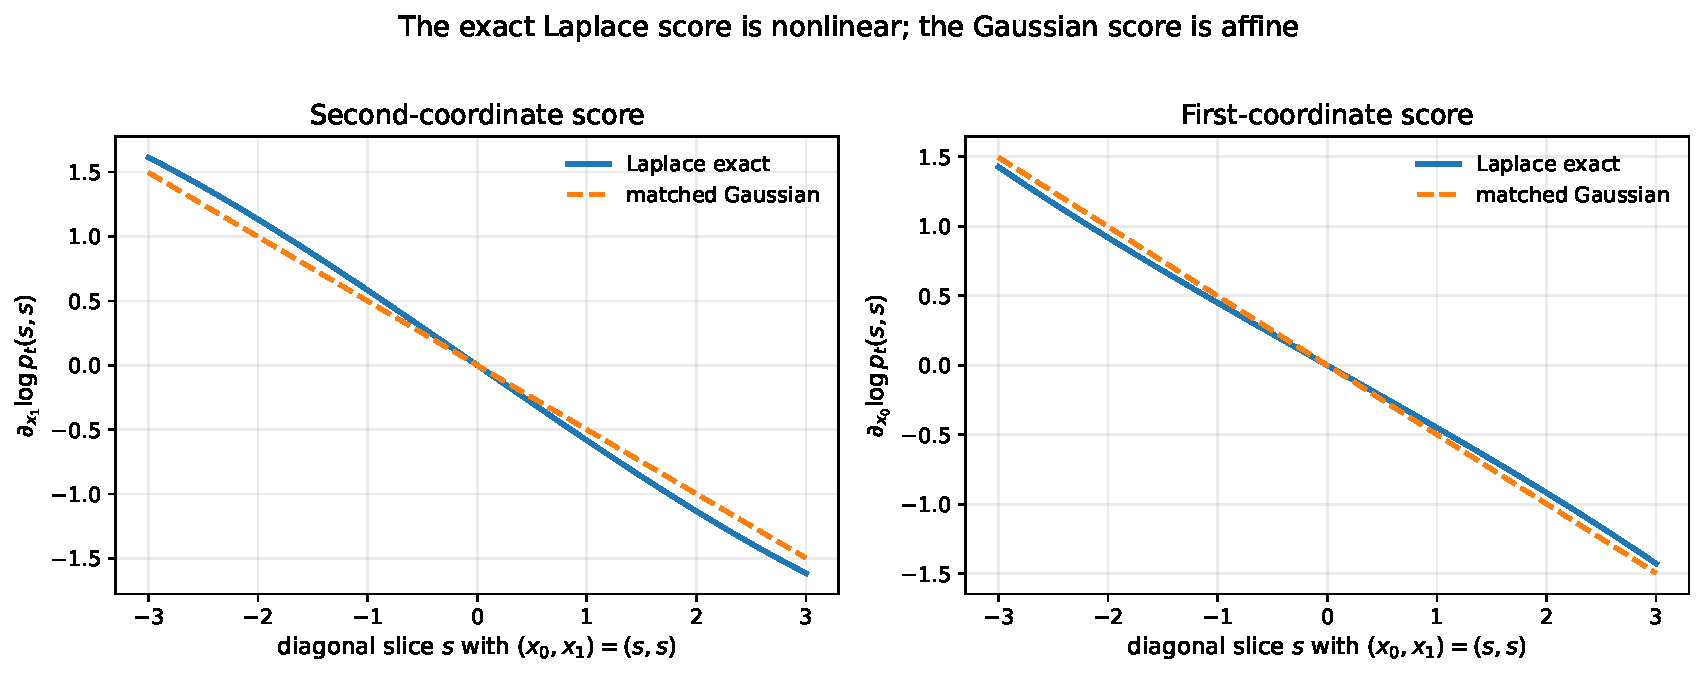
\includegraphics[width=0.94\textwidth]{fig02_score_slices.pdf}
\caption{\textbf{Score slices.} Along the diagonal slice $(x_0,x_1)=(s,s)$, the exact Laplace score is nonlinear, while the matched Gaussian score is affine. This is the first visible signal that the Gaussian benchmark has been left behind.}
\label{fig:score}
\end{figure}

\begin{figure}[t]
\centering
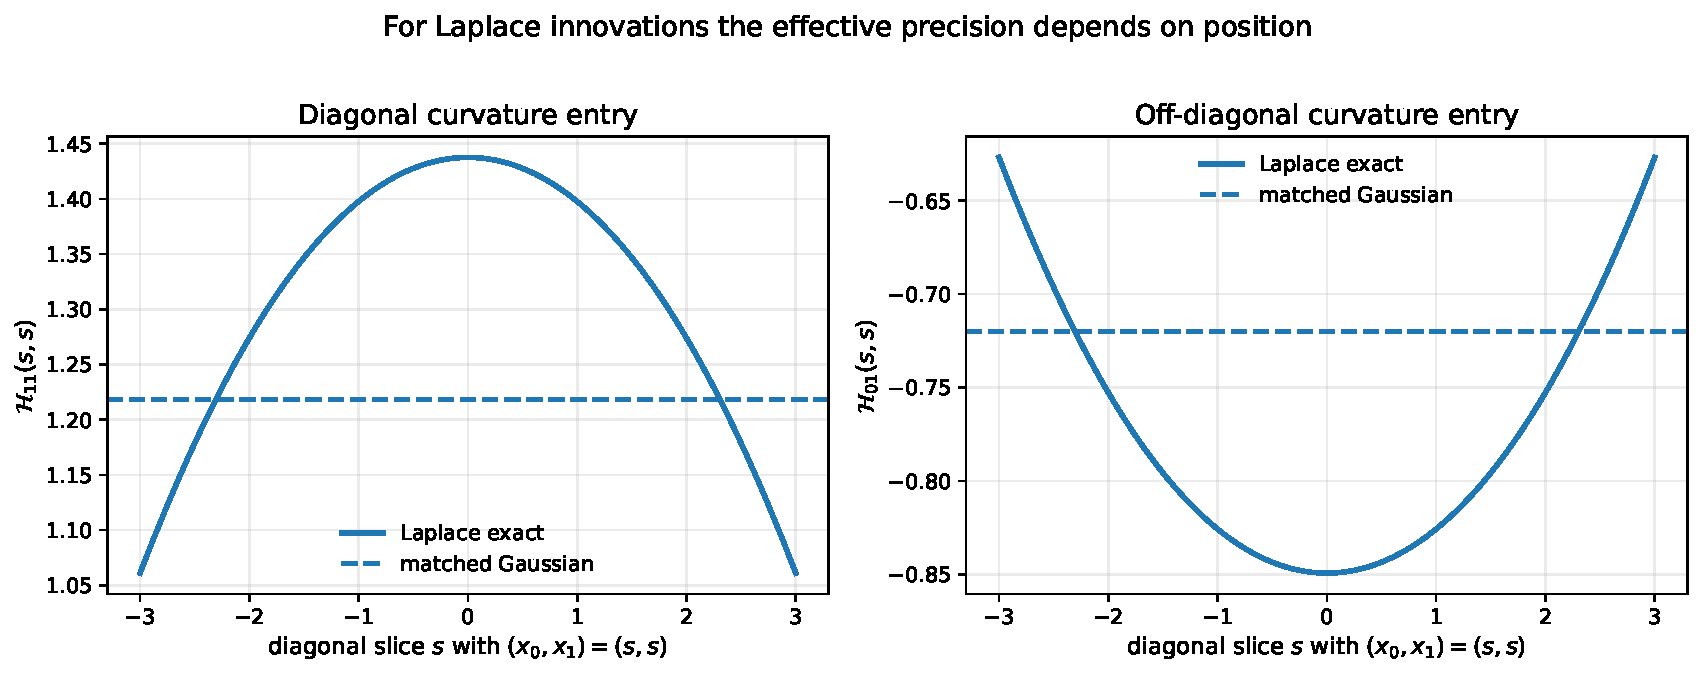
\includegraphics[width=0.94\textwidth]{fig03_hessian_diagonal.pdf}
\caption{\textbf{Curvature on the diagonal slice.} Along $(x_0,x_1)=(s,s)$, both the diagonal and the off-diagonal entries of $\Ht(s,s)$ vary with $s$. In the matched Gaussian model the corresponding entries are constant.}
\label{fig:diag-hessian}
\end{figure}

\begin{figure}[t]
\centering
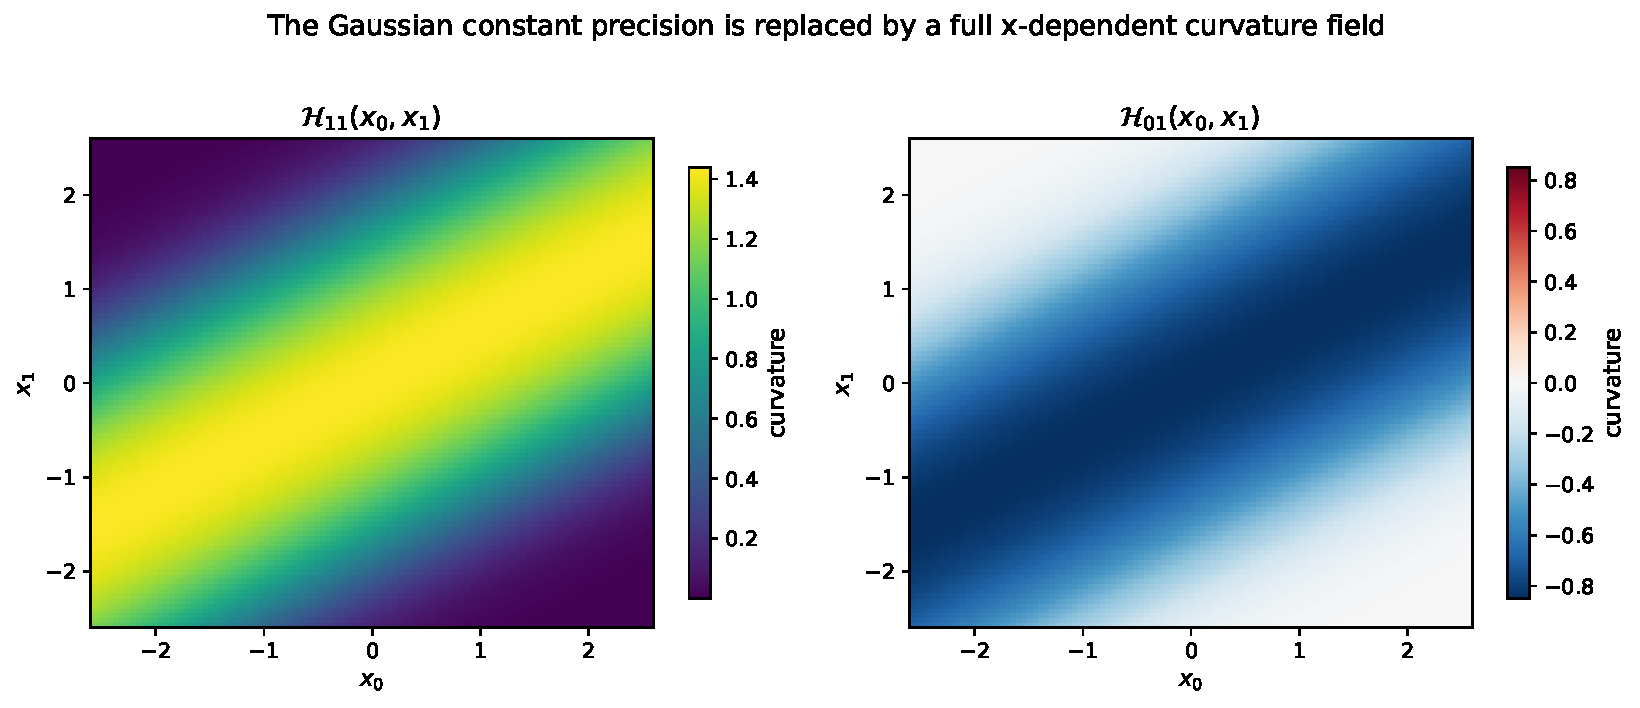
\includegraphics[width=0.94\textwidth]{fig04_hessian_heatmaps.pdf}
\caption{\textbf{Two-dimensional curvature field.} Heatmaps of the exact entries $(\Ht(x_0,x_1))_{11}$ and $(\Ht(x_0,x_1))_{01}$. The Gaussian notion of one fixed precision matrix is replaced by an $x$-dependent field.}
\label{fig:heatmaps}
\end{figure}

\section{Conclusion on the hypotheses}

\begin{enumerate}[leftmargin=1.45em,itemsep=0.35em]
\item \textbf{Finite-time smoothing does not erase non-Gaussianity.} Equation \eqref{eq:cf-laplace} shows that the diffused Laplace law is not Gaussian for any finite $t$.
\item \textbf{The first robust signal is $x$-dependent curvature.} Equations \eqref{eq:H11}--\eqref{eq:H00} give exact formulas for $\Ht(x)$, and Figures \ref{fig:diag-hessian}--\ref{fig:heatmaps} show the variation directly.
\item \textbf{The old $K=2$ closed-form claim is not retained.} The corrected statement is weaker: $K=2$ has an exact nested integral representation, but the previous draft did not establish an elementary closed form comparable to \eqref{eq:exact-density}.
\end{enumerate}

The presentation message is therefore short and clean:
\[
\text{Gaussian benchmark} \Longrightarrow \text{constant } Q_t,
\qquad
\text{Laplace benchmark} \Longrightarrow \text{exact } \mathcal{H}_t(x) \text{ depending on } x.
\]
That is the main signal to present.

\end{document}
